\begin{appendices}
\startcontents[chapters]

\chapter{Additional Figures}
\section{Register Set Multiplex}
\begin{figure}[H]
\centering
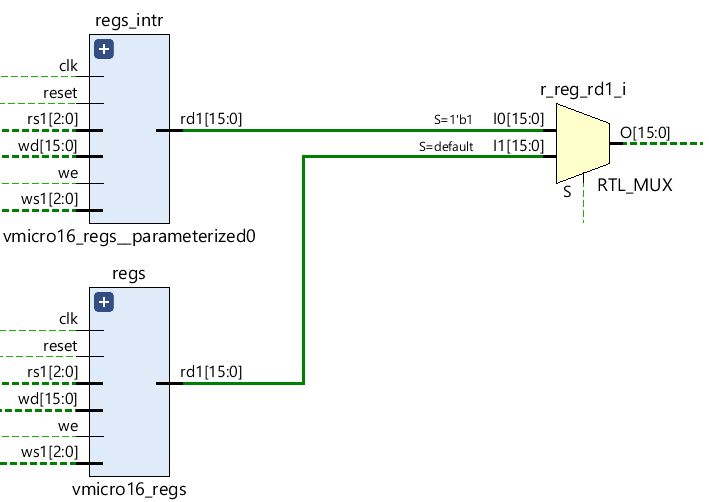
\includegraphics[width=0.7\textwidth]{interrupt_mux}
\caption{Normal mode and interrupt mode register sets are multiplexed to instantly save the context.}
\label{fig:regmult}
\end{figure}


\section{Instruction Set Architecture}
\begin{figure}[H]
\centering
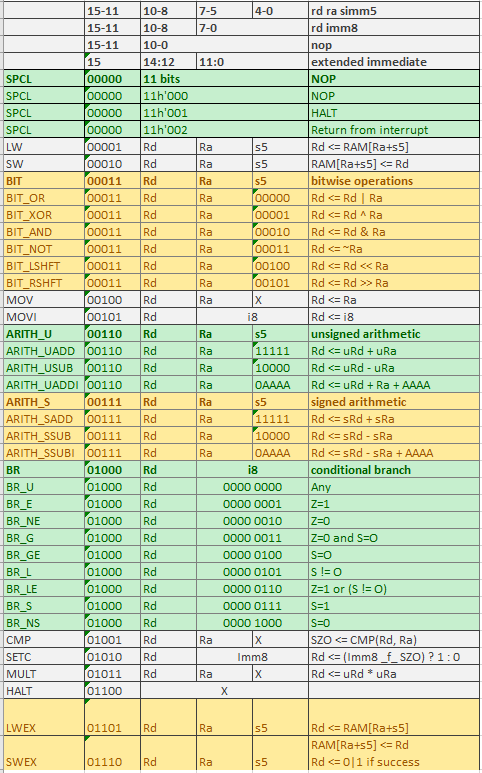
\includegraphics[width=0.7\textwidth]{isa2}
\caption{Vmicro16 instruction set architecture.}
\label{fig:isa}
\end{figure}

\chapter{Configuration Options}
\label{sect:config}
\startcontents[chapters]
\printcontents[chapters]{}{1}{}

\noindent\\
The following configuration options are defined in \verb|vmicro16_soc_config.v|.

\section{System-on-chip Configuration Options}
\begin{table}[H]
\centering
\label{tab:isa}
\begin{tabularx}{\textwidth}{l|l|p{8cm}}
Macro      & Default & Purpose                         \\ 
\hline
CORES  & 4       & Number of CPU cores in the SoC  \\
SLAVES & 7       & Number of peripherals  \\    
DEF\_USE\_WATCHDOG &  & Enable watchdog module to detect deadlocks and infinite loops \\    
\end{tabularx}
\caption{SoC Configuration Options}
\end{table}

\section{Core Options}
\begin{table}[H]
\centering
\begin{tabular}{l|l|p{8cm}}
Macro                      & Default & Purpose                                     \\ 
\hline
DATA\_WIDTH                & 16      & Width of CPU registers in bits              \\
DEF\_CORE\_HAS\_INSTR\_MEM & //      & Enable a per core instruction memory cache  \\
DEF\_MEM\_INSTR\_DEPTH     & 64      & Instruction memory cache per core           \\
DEF\_MEM\_SCRATCH\_DEPTH   & 64      & RW RAM per core                             \\
DEF\_ALU\_HW\_MULT        & 1       & Enable/disable HW multiply (1 clock)        \\
FIX\_T3                    & //      & Enable a T3 state for the APB transaction \\

DEF\_GLOBAL\_RESET           & //      & Enable synchronous reset logic \\

DEF\_USE\_REPROG           & //      & Programme instruction memory via UART0. Requires DEF\_GLOBAL\_RESET\\
\end{tabular}
\caption{Core Options}
\label{tab:isa}
\end{table}

\section{Peripheral Options}
\begin{table}[H]
\centering
\begin{tabular}{l|l|l}
Macro              & Default  & Purpose                                              \\ 
\hline
APB\_WIDTH         &          & AMBA APB PADDR signal width                          \\
APB\_PSELX\_GPIO0  & 0        & GPIO0 index                                          \\
APB\_PSELX\_UART0  & 1        & UART0 index                                          \\
APB\_PSELX\_REGS0  & 2        & REGS0 index                                          \\
APB\_PSELX\_BRAM0  & 3        & BRAM0 index                                          \\
APB\_PSELX\_GPIO1  & 4        & GPIO1 index                                          \\
APB\_PSELX\_GPIO2  & 5        & GPIO2 index                                          \\
APB\_PSELX\_TIMR0  & 6        & TIMR0 index                                          \\
APB\_BRAM0\_CELLS  & 4096     & Shared memory words                                  \\
DEF\_MMU\_TIM0\_S  & 16'h0000 & Per core scratch memory start/end address            \\
DEF\_MMU\_TIM0\_E  & 16'h007F & "                                                    \\
DEF\_MMU\_SREG\_S  & 16'h0080 & Per core special registers start/end address         \\
DEF\_MMU\_SREG\_E  & 16'h008F & "                                                    \\
DEF\_MMU\_GPIO0\_S & 16'h0090 & Shared GPIOn start/end address                       \\
DEF\_MMU\_GPIO0\_E & 16'h0090 & "                                                    \\
DEF\_MMU\_GPIO1\_S & 16'h0091 & "                                                    \\
DEF\_MMU\_GPIO1\_E & 16'h0091 & "                                                    \\
DEF\_MMU\_GPIO2\_S & 16'h0092 & "                                                    \\
DEF\_MMU\_GPIO2\_E & 16'h0092 & "                                                    \\
DEF\_MMU\_UART0\_S & 16'h00A0 & Shared UART start/end address                        \\
DEF\_MMU\_UART0\_E & 16'h00A1 & "                                                    \\
DEF\_MMU\_REGS0\_S & 16'h00B0 & Shared registers start/end address                   \\
DEF\_MMU\_REGS0\_E & 16'h00B7 & "                                                    \\
DEF\_MMU\_BRAM0\_S & 16'h1000 & Shared memory with global monitor start/end address  \\
DEF\_MMU\_BRAM0\_E & 16'h1FFF & "                                                    \\
DEF\_MMU\_TIMR0\_S & 16'h0200 & Shared timer peripheral start/end address            \\
DEF\_MMU\_TIMR0\_E & 16'h0202 & "                                                   
\end{tabular}
\caption{Peripheral Options}
\label{tab:isa}
\end{table}

\clearpage
\chapter{Code Listing}
\startcontents[chapters]
\printcontents[chapters]{}{1}{}

\section{vmicro16\_soc\_config.v}
Configuration file for configuring the vmicro16\_soc.v and vmicro16.v features.

\inputminted[
    linenos,
    fontsize=\scriptsize,
    baselinestretch=0.8,
]{verilog}{../../vmicro16/vmicro16_soc_config.v}

\section{top\_ms.v}
Top level module that connects the SoC design to hardware pins on the FPGA.
\inputminted[
    linenos,
    fontsize=\scriptsize,
    baselinestretch=0.8,
]{verilog}{../../vmicro16/top_ms.v}

\section{vmicro16\_soc.v}
\inputminted[
    linenos,
    fontsize=\scriptsize,
    baselinestretch=0.8,
]{verilog}{../../vmicro16/vmicro16_soc.v}


\section{vmicro16\_periph.v}
Various memory-mapped APB peripherals, such as GPIO, UART, timers, and memory.

\inputminted[
    linenos,
    fontsize=\scriptsize,
    baselinestretch=0.8,
]{verilog}{../../vmicro16/vmicro16_periph.v}

\section{vmicro16.v}
Vmicro16 CPU core module.

\inputminted[
    linenos,
    fontsize=\scriptsize,
    baselinestretch=0.8,
]{verilog}{../../vmicro16/vmicro16.v}



\end{appendices}